\documentclass[12pt]{report}
\usepackage{graphicx}
\usepackage[spanish]{babel} % Para separar correctamente las palabras
\usepackage[utf8]{inputenc} % Este paquete permite poner acentos y eñes usando codificación utf-8

% Title Page
\title{Análisis de Identificadores para Abstraer conceptos del Dominio del Problema}
\author{Javier Azcurra\\\\Trabajo Final de Licenciatura en Cs. de la Computación\\\\\\Facultad de Ciencias Físico Matemáticas y Naturales\\Universidad Nacional de San Luis}

%\centering
%
\includegraphics[scale= 0.18]{./unsl_logo.JPG}

\begin{document}
\maketitle

%\renewcommand{\abstractname}{Agradecimientos}
%\begin{abstract}
% Gracias!
%\end{abstract}

%\tableofcontents %Genera el indice

\begin{abstract}
Las demandas actuales en el desarrollo del software implican una evolución y mantenimiento constante del mismo con el menor costo de tiempo y de recursos. Pensar en estrategias que faciliten las tediosas tareas que diariamente conllevan al crecimiento de los sistemas nos da incapie a iniciarnos en la investigación de herramientas automatizadas que posibiliten el reemplazo del esfuerzo manual que realizan los ingenieros de software a la hora de interpretar un programa.

Estudios indican que los identificadores abundan en los códigos de programas y poseen información relevante detrás de sus abreviaturas por lo tanto no debe ser pasados por alto su análisis a la hora de elaborar herramientas automatizadas de interpretación de códigos.
El correspondiente trabajo habla de técnicas basadas en el análisis de identificadores en códigos escritos en lenguaje JAVA\texttrademark .
Las técnicas de análisis constan de dos etapas la primera consiste en la división de las distintas abreviaturas que componen un identificador y la segunda etapa se encarga en la expansión “semántica” de cada abreviatura capturada en la etapa previa, es decir, expandir las abreviaciones en palabras completas. Para lograr esta expansión se utilizan distintas fuentes semánticas comentarios, literales y documentación o bien fuera del sistema basándose en diccionarios. Algunas estrategias de análisis de identificadores se implementaron en la herramienta \textit{Identifier Analyzer} (IDA) donde se emplearon técnicas de compilación para extraer la información estática y analizar los identificadores con el objeto de poder comparar el desempeño de las estrategias y arribar a conclusiones.


\end{abstract}

\chapter{Introducción}
\section{Problema}

La ingeniería de software contiene tres temáticas muy importantes en desarrollo de los sistemas: el \textit{mantenimiento del software}, \textit{la evolución del software} y la \textit{migración del software}. Para que puedan llevar a cabo sus iniciativas los tres necesitan interpretar previamente el sistema que se esta desarrollando.

La etapa de mantenimiento es importante en el desarrollo de un software ya que este esta sujeto a cambio y a una permanente evolución\cite{PFT02}.
Es común también que por la constate actualización de los sistemas operativos, los motores de base de datos y demás sistemas externos que interactúan con el software desarrollado entren en conflicto, por eso en la fase de mantenimiento también se debe ir actualizando los distintos componentes del producto para una mejor compatibilidad.\cite{RSPMGH02}. Por lo antedicho entre otras diversas razones indican que el mantenimiento del software consume mucho esfuerzo y dinero. Es necesario pensar en estrategias de automatización que puedan ser aplicadas en fases del mantenimiento del software que ayuden a reducir estos costos, para lograrlo se requiere una comprensión del objeto que se va a modificar antes de realizar algún cambio que sea de utilidad.


Los sistemas complejos evolucionan con el tiempo, los nuevos usuarios y requisitos durante el desarrollo del mismo causan que el producto final posiblemente no sea el que se planteó en un comienzo. 
Generalmente los ingenieros del software utilizan modelos de procesos conocidos que se diseñan de antemano para adaptarse a un producto que evoluciona con el tiempo, estos modelos se conocen con el nombre de modelos evolutivos o modelos iterativos, este ultimo hace referencia a que el ingeniero del software pueda obtener una versión entregable del producto cada vez más completa en cada iteración, esto se considera importante ya que las fechas ajustadas y el mercado competitivo obligan a entregar una versión funcional limitada lo más rápido posible y no esperar a tener una única versión completa al final del proceso de desarrollo\cite{RSPMGH02}.
La evolución del software básicamente se atribuye al crecimiento de los sistemas, es decir, tomar una versión operativa y generar una nueva versión ampliada, para lograrlo se necesita una previa interpretación del sistema.


La migración del software es una tarea fundamental y compleja dentro del mantenimiento del software. El objetivo es convertir un viejo sistema dentro de una nueva tecnología sin cambiar la funcionalidad del mismo, lograr esto es costoso \cite{WHAFVR11}. Es fundamental lograr una buena comprensión del sistema antiguo, una forma de alcanzarlo es elevar el código antiguo a un nivel más alto de abstracción tomando las principales características \cite{MMFAF07}.

%WICC:
Todos los problemas a los que se enfrentan los desarrolladores de software el primordial es el de mantener los sistemas en buen funcionamiento \cite{VMAVA95}. 
Esta tarea es imposible de llevar a cabo de forma manual debido a que consume 
muchos costos y esfuerzo humano. 
Por esta razón, existe una subárea de la Ingeniería de Software que se  
dedica al desarrollo de técnicas de inspección y comprensión de software. 
Esta área tiene como principal objetivo que el desarrollador logre un entendimiento 
acabado del software de estudio de forma tal de poder modificarlo disminuyendo en lo posible la gran mayoría de costos \cite{BRM10}. 
El área mencionada se conoce en la jerga de la Ingeniería de Software como: 
\textit{Comprensión de Programas (CP)}.


La CP es un área de la Ingeniería de Software cuyo objetivo 
principal es desarrollar métodos, técnicas y herramientas que faciliten al programador 
el entendimiento de las funcionalidades de los sistemas de software.
Una forma de alcanzar este objetivo consiste en relacionar el Domino del Problema, 
es decir la salida del sistema, con el dominio del programa, o sea 
con las partes del programa utilizadas para generar la salida del sistema.
\textbf{La construcción de esta relación representa el principal desafío en el contexto de la CP.}

%==============================================================================


\section{Solución}

\textbf{Una solución posible al desafío previamente mencionado consiste en construir una representación para el dominio del problema y otra para el dominio del programa luego unir ambas representaciones utilizando una estrategia de vinculación} 
Los caminos que conducen a facilitar la vinculación de las dos representaciones consiste en el uso/creación de Herramientas de Comprensión. 
Una Herramienta de Compresión presenta diferentes perspectivas del software que posibilitan que el ingeniero pueda percibir el funcionamiento del sistema. 
Para construir herramientas de comprensión, se deben tener en cuenta tres pilares importantes, ellos son: \textit{Interconexión de Dominios}, 
\textit{Visualización de Software} y 
\textit{Extracción de la Información} \cite{STOREY99,BROOK82}.

La \textit{visualización del software} es una característica importante en la comprensión de programas, básicamente provee una o varias representaciones visuales de algún sistema particular \cite{BRM10}.
Dichas vistas, cuando están bien elaboradas, permiten analizar y percibir la información extraída desde un programa con mayor facilidad.

La \textit{Interconexión de Dominios} \cite{BRM10} tiene como principal objeto de estudio la transformación y vinculación de un dominio específico en otro dominio. 
Este último dominio puede estar en un alto o bajo nivel de abstracción. 
El punto importante es que cada componente de un dominio se vea reflejado en una o más componentes del otro y viceversa. 
A modo de ejemplo, se puede mencionar la transformación de un código fuente Dominio del Programa) en un Grafo de Llamadas a Funciones (Dominio de Grafos). En este contexto existe una amplia gama de transformaciones siendo la más escasa y difícil de conseguir aquella que relaciona el Dominio del Problema con el Dominio del Programa.

Por \textit{Extracción de la Información} se entiende el uso/desarrollo de técnicas que 
permitan extraer información desde el sistema de estudio. 
Esta información puede ser: Estática o Dinámica, dependiendo de las necesidades del 
ingeniero de software o del equipo de trabajo.
Para la extracción de la información estática se utilizan técnicas de compilación tradicionales, que se encargan de recuperar información de cada componente del sistema. Todas las actividades que forman parte de esta tarea se realizan desde el código fuente sin ejecutar el sistema. Generalmente, en este tipo de trabajos se construye un analizador sintáctico con las acciones semánticas necesarias para extraer la información requerida.
Por otro lado la extracción dinámica de información del sistema se obtiene  
aplicando técnicas de instrumentación de código, estas técnicas consisten en insertar sentencias dentro del código fuente del sistema con el fin de recuperar las partes del programa que se utilizaron para 
producir la salida. 
La principal diferencia que radica entre ambas técnicas es que las dinámicas requieren que el sistema se ejecute, mientras que las estáticas esto no es necesario.

Los párrafos precedentes permiten percibir la importancia de las técnicas de 
\textbf{extracción de la información}. 
Sin ellas no sería posible la construcción de visualizaciones y técnicas de 
interconexión de dominios\cite{BRM10}. 

\textbf{Concluimos que tanto la representación del dominio del problema como la representación del dominio del programa se construye en base a la información, estática y dinámica, que se extrae de los mismos. 
La estrategia de vinculación usa esa información para construir un mapeo entre los elementos de ambos dominios.}
Por esta razón, en este trabajo se describe una línea de investigación que tiene 
como principal foco de estudio el análisis, la creación y elaboración de técnicas de extracción de la información estática de los sistemas de software que permitan aproximar a la construcción de la relación entre el Dominio del Problema y el Dominio del Programa.
Finalmente, es importante mencionar que la información dinámica es tan importante como la información estática, sin embargo su extracción requiere del estudio de otro tipo de aproximaciones que conforman en sí otra línea de investigación.


Actualmente, existen muchas herramientas de comprensión que basan sus análisis en componentes que están presentes en la información estática de los códigos de programas, alguno de ellos son nombres de variables, tipos de las variables,los métodos de un programa orientado a objeto, las variables locales a un método, etc. Estos son elementos que componen la información formal. Sin embargo, a través del estudio del estado del arte, se pudo detectar que son pocas las estrategias de análisis estático que analizan la información informal que se encuentra disponible en el código fuente, por información informal se entiende aquella contenida en 
los: \textit{comentarios de los módulos}, \textit{comentarios de las funciones}, \textit{literales strings}, \textit{documentación} etc.
Esto se debe a que dicha información se encuentra expresada en lenguaje natural y por lo tanto su interpretación escapa del análisis estático y requiere de la aplicación de \textit{Técnicas de Procesamiento de Lenguaje Natural} 
\cite{DCPHJP09,TERD01}.
Este trabajo se centra en los \textit{identificadores} ids como fuente principal de información. Detrás de los ids se encuentra oculta información que es propia del dominio del problema. Generalmente los ids están compuestos por más de una palabra en forma de abreviatura, una posibilidad para exponer la información oculta consiste en traducir estas abreviaturas en las correspondientes palabras expresadas en lenguaje natural.

Una aproximación a la solución de este problema es tomar los ids, 
aplicarles técnicas de división o separación y luego técnicas de expansión a las 
abreviaturas para transformar las mismas en palabras completas. 
Para lograr esto, primero se descompone al identificador en las distintas palabras 
abreviadas que lo componen, luego se toma cada abreviatura y se expande a la palabra completa.

La dificultad que presenta esta técnica es que normalmente los nombres de los ids se basan en función de la idiosincrasia del 
programador \cite{LFBEX07, EHPV09}
y esto representa un problema para el traductor. Otro problema a tener en cuenta es que las abreviaturas representan palabras en lenguaje natural, el cual es ambiguo y puede generar controversia en la conversión.

Por lo tanto es necesario la ayuda de fuentes que contengan información informal presentes en el código que ayuden a la interpretación de los ids. Los candidatos serios a lograr este cometido son comentarios y los literales string.
Sin duda, los comentarios tienen como principal finalidad ayudar a 
entender un segmento de código \cite{JDPH08}.
Dicho de otra manera, son una fuente importante de información de 
los conceptos del Dominio del Problema. 
Por esta razón, se puede ver a los comentarios como una herramienta 
natural para entender el significado de los ids de un código,
como así también el funcionamiento del sistema en sí.

Por otro lado para poder entender la semántica de un identificador es analizando los literales o constantes strings.
Estos representan un valor constante formado por  secuencias de caracteres. 
Ellos son generalmente utilizados en la muestra de carteles por pantalla, y 
comúnmente se almacenan en variables de tipo \textit{string} (como es el caso de 
los programas escritos en Java).
Tanto los literales como los comentarios están escritos en lenguaje natural, por lo tanto es un desafío su correcta interpretación.
Detrás de la información informal se oculta información relevante del 
Dominio del Problema.
Esta información es muy importante porque facilita  la reconstrucción de la relación del  
Dominio del Problema con el Dominio del Programa 
\cite{DWE04}.

En este trabajo se buscan estrategias basadas en el análisis de los ids que faciliten la comprensión de programas haciendo así un pequeño aporte en la solución a la problemática de vincular ambos dominios mencionados: 

\begin{itemize}

\item Se investigaron herramientas de construcción de Analizadores Léxicos y Analizadores Sintácticos que emplean la teoría asociada a las gramáticas de atributos. 
De la investigación mencionada previamente,  
se determinó que la herramienta \textit{ANTLR}\footnote[1]{http://www.antlr.org/} es la más adecuada para extraer eficazmente los ids y toda la información relevante asociada a ellos que facilite su análisis.

\item Se construyó un analizador sintáctico del lenguaje Java que permite extraer los ids, comentarios y literales encontrados en el código fuente del sistema de estudio.

\item  Se estudiaron y se implementaron las técnicas de división de ids Greedy, Random \cite{HDD06,FBL06} que se encargan de separar a los ids en partes, donde cada parte representa una palabra abreviada.

\item Se investigaron y se implementaron técnicas de expansión de ids en donde las abreviaturas previamente divididas se expanden en palabras completas.  
Dichas técnicas llevan a disponer de listas de palabras formadas de los comentarios y literales capturados, (como así también una lista de palabras del diccionario en español).

\item Se implementó una herramienta \textit{Identifier Analyzer} (IDA) que permite visualizar los atributos (ambiente, tipo de identificador, número de línea,etc) de cada objeto mostrando la parte del código donde se encuentra ubicados. Se incorporó en la implementación ademas las técnicas mencionadas en los ítems anteriores usando \textit{ANTLR} como herramienta soporte para la extracción de información.

\end{itemize}


%======================================================================

\pagebreak %salto de pagina
\section{Contribución}
La línea de investigación descrita en este trabajo final se encuentra enmarcada en el 
contexto del proyecto: \textit{Ingeniería del Software: Conceptos Métodos Técnicas y 
Herramientas en un Contexto de Ingeniería de Software en Evolución} de la Universidad 
Nacional de San Luis. 
Dicho proyecto, es reconocido por el programa de incentivos y es la continuación de 
diferentes proyectos de investigación de gran éxito a nivel nacional e internacional.

También se forma parte del proyecto bilateral entre la Universidade do Minho (Portugal)
 y la Universidad Nacional de San Luis (Argentina) denominado \textit{Quixote: Desarrollo de 
Modelos del Dominio del Problema para Inter-relacionar las Vistas Comportamental y 
Operacional de Sistemas de Software}. Quixote\footnote[2]{http://www3.di.uminho.pt/~gepl/} fue aprobado por el 
Ministerio de Ciencia, Tecnología e Innovación Productiva de la Nación 
(MINCyT) y la Fundação para a Ciência e Tecnología (FCT) de Portugal. 
Ambos entes soportan económicamente la realización de diferentes misiones de investigación desde Argentina a Portugal y viceversa.

\section{Organización de Trabajo Final}
En este trabajo final se presenta una línea de investigación que se centra en el estudio, 
creación e implementación de técnicas de extracción de la información estática desde 
los sistemas de software. 
Esta información puede ser estrictamente relacionada con el código del programa, 
o bien con la información informal provista por los programadores a través de 
comentarios, literales y documentación. El trabajo esta organizado de la siguiente manera. El capítulo 2 define conceptos teóricos relacionados a la comprensión de programas, cuales son las necesidades que implica su estudio y que soluciones presenta en la vida del desarrollo del software. El capítulo 3 habla de técnicas de análisis de identificadores y que fuentes semánticas son utilizadas para su interpretación. El capítulo 4 trata sobre la herramienta \textit{Identifier Analyzer} (IDA) que implementa algunas técnicas de análisis de identificadores sobre códigos escritos en JAVA\texttrademark ademas de algunos casos de estudio. El capítulo 5 menciona las conclusiones elaboradas y posibles trabajos futuros.

\chapter{Comprensión de Programas}
\section{Introducción}
La CP es un área de la Ingeniería de Software que tiene como meta primordial desarrollar métodos, técnicas y herramientas que ayuden al programador a comprender en profundidad los sistemas de software. La principal ventaja es que la CP reduce el esfuerzo y los costos en la etapas de mantenimiento y la evolución del software esto se logra abstrayendo la información contenida en el código a un nivel mas alto y de esta manera esclarecer mas su interpretación.\cite{MPMR07}
%NECESITO HABLAR DE INGENIERIA INVERSA???
%BUSCAR MAS MATERIAL CON DATOS ESTADISTICOS???
Diversos estudios e investigaciones demuestran que el principal desafío esta enmarcado en vincular el dominio del problema y el dominio del programa. El primero se refiere al resultado de la ejecución del sistema, mientras que el segundo indica todos los componentes involucrados que causaron dicho resultado. En la figura 2.1 se muestra gráficamente el principal objetivo que es vincular ambos dominios. El inconveniente es que esta relación real es compleja de llevar a cabo y para facilitar la tarea se reconstruye utilizando aproximaciones nombradas como representación del problema y representación del programa correspondiente a cada dominio mas una estrategia de vinculación que simula ser la relación real.

\begin{figure}[h] %[h] para here [b] para bottom [t] para top
\centering
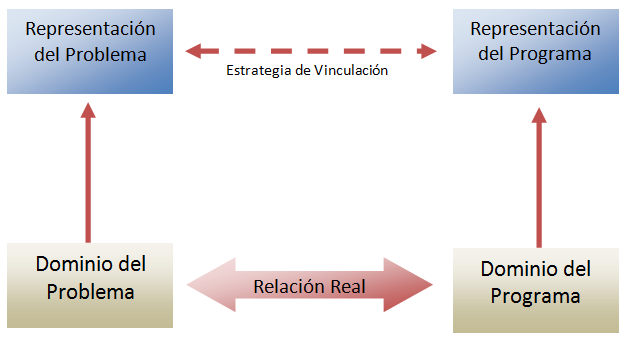
\includegraphics[scale= 0.25]{./dom.png}
\caption{Gráfico de Comprensión de Programas}
\end{figure} \label{captura1}

El procedimiento que se lleva cabo para armar la estrategia de vinculación implica primero tener ambas representaciones de los dominios. 
Al elaborar estas representaciones se deben tener en cuenta conceptos muy importantes que son cimientos sobre los cuales esta sustentada la CP: la visualización de software, la extracción de información y la interconexión de dominios.

\section{Visualización de Software}

La visualización de software es un área de la ingeniería de software dedicada a la construcción de representaciones visuales de los sistemas. 

Esta representaciones conocidas con el nombre de vistas se encargan de brindar información del sistema de estudio para ayudar la comprensión. Existen distintos tipos de vistas, en si mismo, la primer vista de un sistema es el código donde la información no esta tan clara para un desarrollador ajeno sobre todo si el software es grande y complicado. Es por eso que se necesita recurrir a otras vistas o perspectivas del sistema.
Los sistemas de visualización (SV) de software son herramientas útiles que se encargan de analizar los distintos módulos de un programa y generar vistas, dependiendo de la información que se desea visualizar existe una vista especifica\cite{MPMR07}. Cabe recordar que la información concebida en un sistema puede ser estática o dinámica.

Para la construcción de vistas se requieren un conjunto de librerías gráficas. Las librerías gráficas son programas que simplifican la elaboración de las vistas. Cada librería posee distintas características y el programador tiene la tarea de elegir cual es la librería mas adecuada para la vista que desea construir.


Después de investigar distintos SV que actualmente existen: Myers, Price, Roman and Kenneth, Storey\cite{MBPHRU10} %tesis del mario falta!!!
en donde se concluye que la mayoría apuntan a capturar conceptos situados solo en el dominio del programa restando importancia al dominio del problema y a la relación entre ambos dominios. Debido a esta falencia Berón propone\cite{MBPHRU10} %tesis del mario falta!!!
SV orientados a la CP ampliando aun mas los sistemas que hoy por hoy ya existen.

\section{Extracción de Información}

Siguiendo con el objetivo principal que es aproximarse en la construcción de relación del dominio del problema con el dominio programa a través de representaciones esta requiere la extracción de información de ambos dominios. En la ingeniería del software existe una temática que se encarga de desarrollar técnicas y métodos para la extracción de la información en códigos de los sistemas, estas técnicas están catalogadas según el tipo de información que extraen.

La información estática esta contenida en el código fuente del sistema 
tipos, identificadores, procedimientos, y demás componentes visibles forman parte de ella. Una estrategia utilizada para extraer esta información es elaborar un analizador sintáctico que posea acciones semánticas especificas para extraer los datos deseados del código sin necesidad de ejecutar el programa. 

La información dinámica se basa en elementos del programa presentes durante la ejecución del sistema. Para la extracción de este tipo de información se procede a bosquejar una técnica de instrumentación de código la cual consiste en aplicar sentencias en el código sin modificar su semántica así cuando el sistema sea ejecutado las sentencias que se insertaron retornen los elementos que se emplearon para generar la salida de la ejecución.


requiere que el sistema sea modificado sin cambiar su semántica y luego ejecutado.


%\section{Interconexión de dominios}
%\section{Comentarios}



%========================================================================
\bibliographystyle{plain}%{alpha}
\bibliography{biblo.bib}

\end{document}
